\section{Ứng dụng ma trận trong vật lý và cơ học}\label{sec_1}

Mục tiêu của phần này là sử dụng các tính chất của ma trận để tìm lại các kết quả đã trình bày trong tuần trước. Các kết quả trình bày dưới đây hoàn toàn có thể áp dụng được cho các hệ thống dao động phức tạp có nhiều bậc tự do hơn. Về mặt toán học hệ dao động 2 bậc tự do với các hệ dao động có 3,4,5 hoặc thậm chí 100 bậc tự do là tương tự.

\subsection{Làm quen với ma trận trong cơ học}
\subsubsection{Dao động tự do}

Để làm quen với các khái niệm mới và ôn lại các phép toán ma trận, chúng ta sẽ sử dụng lại ví dụ về hệ dao động 2 bậc tự do đã trình bày trong tuần trước \cref{fig_2dofs}.

\begin{figure}[htbp]
    \centering
    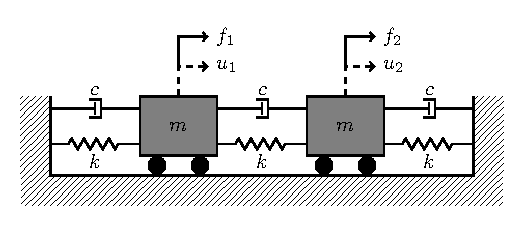
\includegraphics[width=1.\textwidth]{Tuan6/figure/mass_spring_damper_2dofs.pdf}
    \caption{2 dofs system}
    \label{fig_2dofs}
\end{figure}

Điều đầu tiên trong khảo sát một hệ thống dao động như trên hình đó là xác định các modes dao động riêng của hệ. Các modes dao động riêng của hệ là các modes mà ở đó tất cả các bậc tự do biến thiên theo thời gian với cùng tần số. Vì đây là một hệ thống tuyến tính nên nghiệm tổng quát (bất kỳ chuyển động nào của hai khối lượng) sẽ được thể hiện dưới dạng tổ hợp tuyến tính của các nghiệm liên quan đến từng chế độ. Để xác định các modes dao động riêng, ta bắt đầu với việc khảo sát hệ trong chế độ dao động tự do. Có nghĩa là $c=0$ và $f_1=f_2=0$. Ta có phương trình cân bằng cho hệ bên trên.

\begin{equation}\label{eq_PT2dofs}
    \begin{cases}
        m \ddot{u}_1 + 2ku_1 - ku_2 = 0 \\
        m \ddot{u}_2 + 2ku_2 - ku_1 = 0 \\
    \end{cases}
\end{equation}

Biểu diễn dưới dạng mà trận

\begin{equation}
    \label{eq_PTmatrix}
    \underbrace{\begin{bmatrix}
        m & 0\\ 0 & m
    \end{bmatrix}}_{\bf M}\underbrace{\begin{bmatrix}
        \ddot{u}_1 \\ \ddot{u}_2
    \end{bmatrix}}_{\ddot{\bf u}} +\underbrace{\begin{bmatrix}
        2k & -k \\ -k & 2k
    \end{bmatrix}}_{\bf K} \underbrace{\begin{bmatrix}
        u_1 \\ u_2
    \end{bmatrix}}_{\bf u} = \underbrace{\begin{bmatrix}
        0 \\ 0
    \end{bmatrix}}_{\bf O} 
\end{equation}

Các bậc tự do dao động với cùng sự phụ thuộc theo thời gian nên chúng ta có:

\begin{equation}
    {\bf u} = \begin{bmatrix}
        u_1 \\ u_2
    \end{bmatrix} = {\bf X}cos(\Omega t)
\end{equation}

Thay vào PT \cref{eq_PTmatrix} ta có:

\begin{equation}
    {\bf K}{\bf X} - \Omega^2{\bf M}{\bf X} = 0 \Leftrightarrow ({\bf K-\Omega^2{\bf M}}){\bf X} = 0
\end{equation}

Đây là một hệ phương trình tuyến tính với vế trái bằng 0. Để có nghiệm khác không, ma trận $\bf K-\Omega^2{\bf M}$ phải suy biến. Nghĩa là định thức của nó phải bằng 0:

\begin{equation}
    det({\bf K}-\Omega^2{\bf M}) = 0
\end{equation}

Đây là bài toán tìm trị riêng và vector riêng cua ma trận. Ta có thể giải bài toán này bằng cách sử dụng các hàm của Python như \textbf{numpy.linalg.eig} hoặc \textbf{scipy.linalg.eig}. Tuy nhiên vì đây là một ma trận $2\times 2$ nên ta có thể giải trực tiếp. Trị riêng (hay là tần số riêng) của ma trận này là nghiệm của phương trình bậc 2:

\begin{equation}
    \Omega^2 =  \Omega_1^2 = \frac{k}{m} \quad \hbox{va} \quad \Omega^2 = \Omega_2^2 = \frac{3k}{m}
\end{equation}

Vector riêng của hệ là

\begin{equation}
    {\bf X} = {\bf X}_1 = \begin{bmatrix}
        1 \\ 1
    \end{bmatrix} \quad \hbox{va} \quad {\bf X} = {\bf X}_2 = \begin{bmatrix}
        1 \\ -1
    \end{bmatrix}
\end{equation}

Nghiệm tổng quát của hệ là tổ hợp tuyến tính của hai modes này. Ta có thể viết lại nghiệm tổng quát của hệ như sau:

\begin{equation}
    {\bf u}=\underbrace{\left(A_1 \cos \left(\Omega_1 t\right)+B_1 \sin \left(\Omega_1 t\right)\right) {\bf X}_1}_{\hbox{Mode 1}}+\underbrace{\left(A_2 \cos \left(\Omega_2 t\right)+B_2 \sin \left(\Omega_2 t\right)\right) {\bf X}_2}_{\hbox{Mode 2}}
\end{equation}

Các hằng số $A_1, B_1, A_2, B_2$ được xác định từ các điều kiện ban đầu của hệ. Ví dụ nếu ta biết vận tốc và vị trí ban đầu của hai khối lượng thì ta có thể xác định được các hằng số này.

\subsubsection{Dao động cưỡng bức - Không có giảm chấn}

Xét trường hợp $f_1 = F_1cos(\omega t)$ va $f_2 = F_2cos(\omega t)$. Đặt ${\bf f} = \begin{bmatrix} F_1 \\ F_2\end{bmatrix}cos(\omega t) = {\bf F}cos(\omega t)$. Nghiệm của PT lúc này có dạng ${\bf u} = \begin{bmatrix} U_1 \\ U_2\end{bmatrix}cos(\omega t) = {\bf U}cos(\omega t)$. Thay vào PT \cref{eq_PTmatrix}, ta có:

\begin{equation}
    -\omega^2{\bf M}{\bf U} + {\bf K}{\bf U} = {\bf F} \Rightarrow {\bf U} = (-\omega^2{\bf M}+{\bf K})^{-1} {\bf F}
\end{equation}

Ta tìm được giá trị của $U_1$ va $U_2$

\begin{equation}
    U_1 = \frac{F_1(2k-m\omega^2)+F_2k}{(k-m\omega^2)(3k-m\omega^2)} \quad \hbox{va} \quad U_2 = \frac{F_1k+F_2(2k-m\omega^2)}{(k-m\omega^2)(3k-m\omega^2)}
\end{equation}

\subsubsection{Dao động cưỡng bức - có giảm chấn}

Trường hợp hệ số giảm chấn  $c \neq 0$, phương trình cân bằng được viết lại như sau:

\begin{equation}\label{eq_PT2dofs_c}
    \begin{cases}
        m \ddot{u}_1 + 2c\dot{u}_1 - c\dot{u}_2 + 2ku_1 - ku_2 = f1 \\
        m \ddot{u}_2 + 2c\dot{u}_2 - c\dot{u}_1 + 2ku_2 - ku_1 = f2 \\
    \end{cases}
\end{equation}

Dạng ma trận của phương trình này là:

\begin{equation}\label{eq_PT2dofs_c_matrix}
    \underbrace{\begin{bmatrix}
        m & 0\\ 0 & m
    \end{bmatrix}}_{\bf M}\underbrace{\begin{bmatrix}
        \ddot{u}_1 \\ \ddot{u}_2
    \end{bmatrix}}_{\ddot{\bf u}} + \underbrace{\begin{bmatrix}
        2c & -c \\ -c & 2c
    \end{bmatrix}}_{\bf C}\underbrace{\begin{bmatrix}
        \dot{u}_1 \\ \dot{u}_2
    \end{bmatrix}}_{\dot{\bf u}} +\underbrace{\begin{bmatrix}
        2k & -k \\ -k & 2k
    \end{bmatrix}}_{\bf K} \underbrace{\begin{bmatrix}
        u_1 \\ u_2
    \end{bmatrix}}_{\bf u} = \underbrace{\begin{bmatrix}
        f_1 \\ f_2
    \end{bmatrix}}_{\bf f} 
\end{equation}

Để giải phương trình này, chúng ta sẽ viết nó về dạng số phức. Vector ngoại lực ${\bf f}$ lúc này sẽ được biểu diễn ở dạng phức ${\bf f} = {\bf F}e^{j\omega t}$. Nghiệm của phương trình sẽ có dạng ${\bf u} = {\bf U}e^{j\omega t}$.

Thay vào phương trình \cref{eq_PT2dofs_c_matrix} ta có (\textcolor{red}{việc biến đổi để suy ra nghiệm dưới đây là một bài tập dành cho các bạn}):

\begin{equation}\label{eq_nghiemphuc}
    \begin{aligned}
        {U}_1 &=\frac{\left(2 F_1+F_2\right) k-F_1 m \omega^2+j c\left(2 F_1+F_2\right) \omega}{\left(j c \omega+k-m \omega^2\right)\left(3 j c \omega+3 k-m \omega^2\right)}\\
        {U}_2 &=\frac{\left(F_1+2 F_2\right) k-F_2 m \omega^2+j c\left(F_1+2 F_2\right) \omega}{\left(j c \omega+k-m \omega^2\right)\left(3 j c \omega+3 k-m \omega^2\right)}
    \end{aligned}
\end{equation}

\textbf{\textcolor{red}{Câu hỏi: chúng ta sẽ giải quyết bài toán như thế nào nếu ${\bf f}$ có dạng ${\bf f} = {\bf F}_1cos(\omega_1t) + {\bf F}_2sin(\omega_2t)$ ?}}

